\begin{withoutheadline}
\begin{frame}
\vspace*{-13mm}
\begin{figure}
	\hspace*{-4.2mm}
    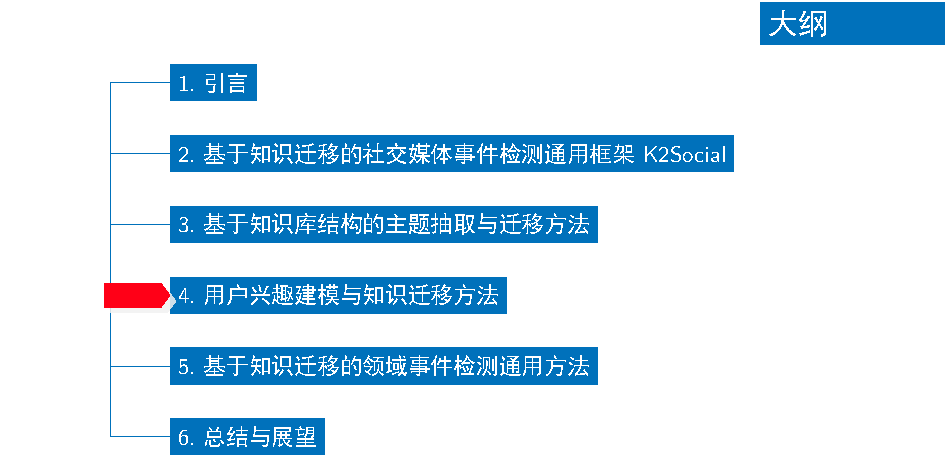
\includegraphics[width=1.0\paperwidth]{img/contents4_output.pdf}
\end{figure}

\end{frame}
\end{withoutheadline}

\section{用户兴趣建模与知识迁移方法}

%------------------------------
%TODO 要说明对突发事件检测有迫切需求
\begin{frame}
\frametitle{Motivation}	
issue
说明对突发事件检测有迫切需求

\pdfnote{前面一节中已经分析了知识迁移对事件检测准确性的提升,这一小节中我们分析知识迁移对事件检测时效性的提升}
\end{frame}

\begin{frame}
\frametitle{突发事件的特点}
这里放一幅插图,说明突发事件的特点是不同兴趣的用户在同一时间窗口内都关心的事件。
\pdfnote{突发事件的特点是不同兴趣的用户在同一时间窗口内都关心的事件。}
\end{frame}

%------------------------------
\begin{frame}
\frametitle{Motivation}
\begin{figure}[h]
		\setlength{\abovecaptionskip}{0.cm}
        \setlength{\belowcaptionskip}{0.cm}
        \centering
		\caption{社交媒体关注网络用于扩充个人自我描述信息示意图}
        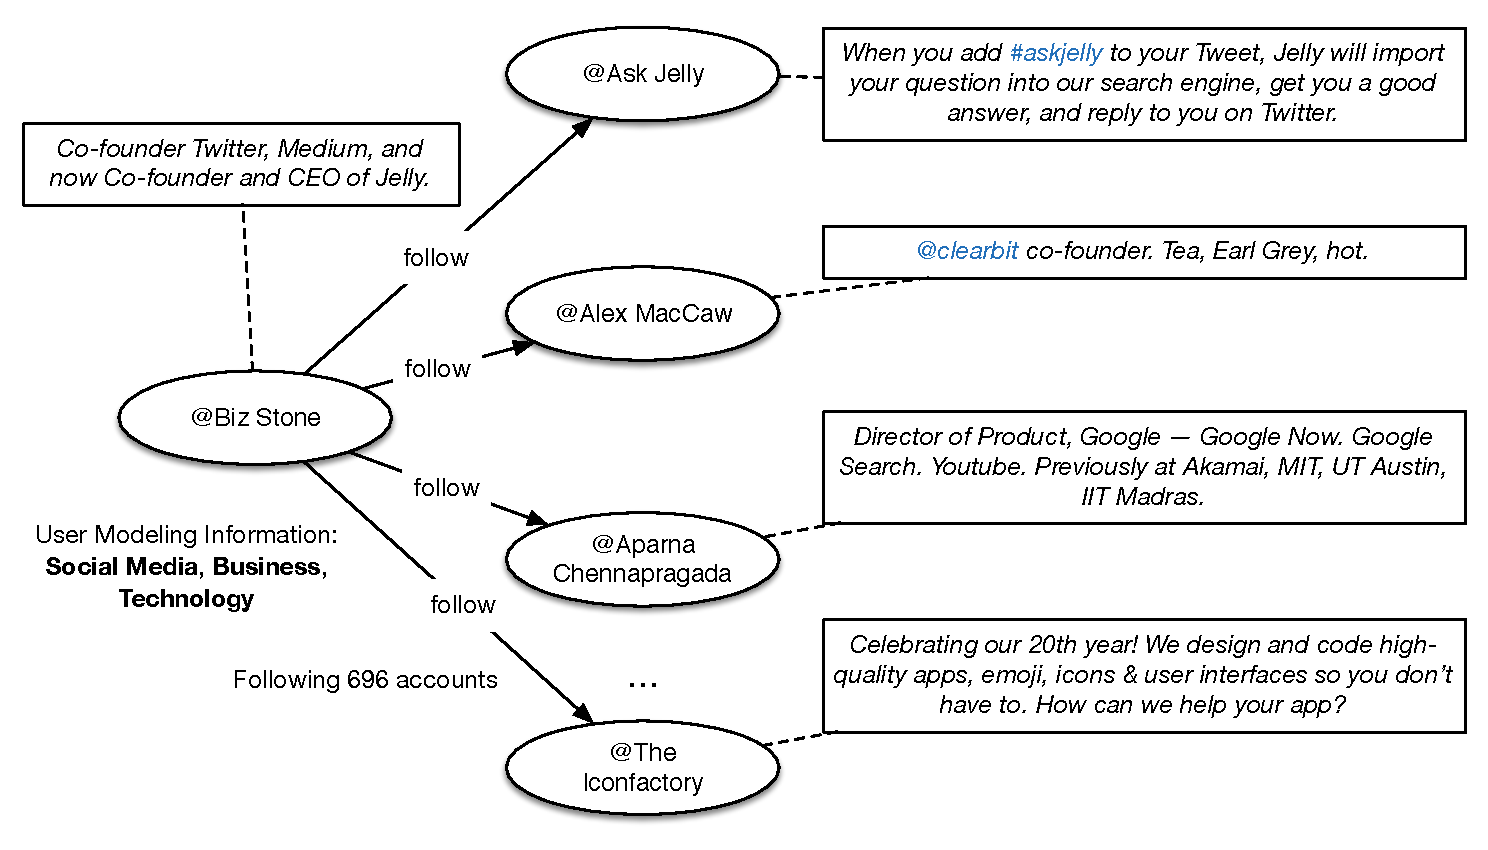
\includegraphics[width=0.9\columnwidth]{img/UMIETM/UMIETM_profile.pdf}
\end{figure}
\end{frame}

%------------------------------
\begin{frame}
\frametitle{我们的方法}
UMIETM模型(User Modeling Based Interest and Event Topic Modeling)
\begin{itemize}
\item 使用用户个人描述信息与用户关注网络建模用户兴趣分布
\item 将用户兴趣知识迁移到微博中
\item 区分用户兴趣与突发事件
\end{itemize}

\vspace{-3mm}
\begin{figure}
	\setlength{\abovecaptionskip}{0.cm}
	\setlength{\belowcaptionskip}{0.cm}
	\caption{UMIETM概率模型}
	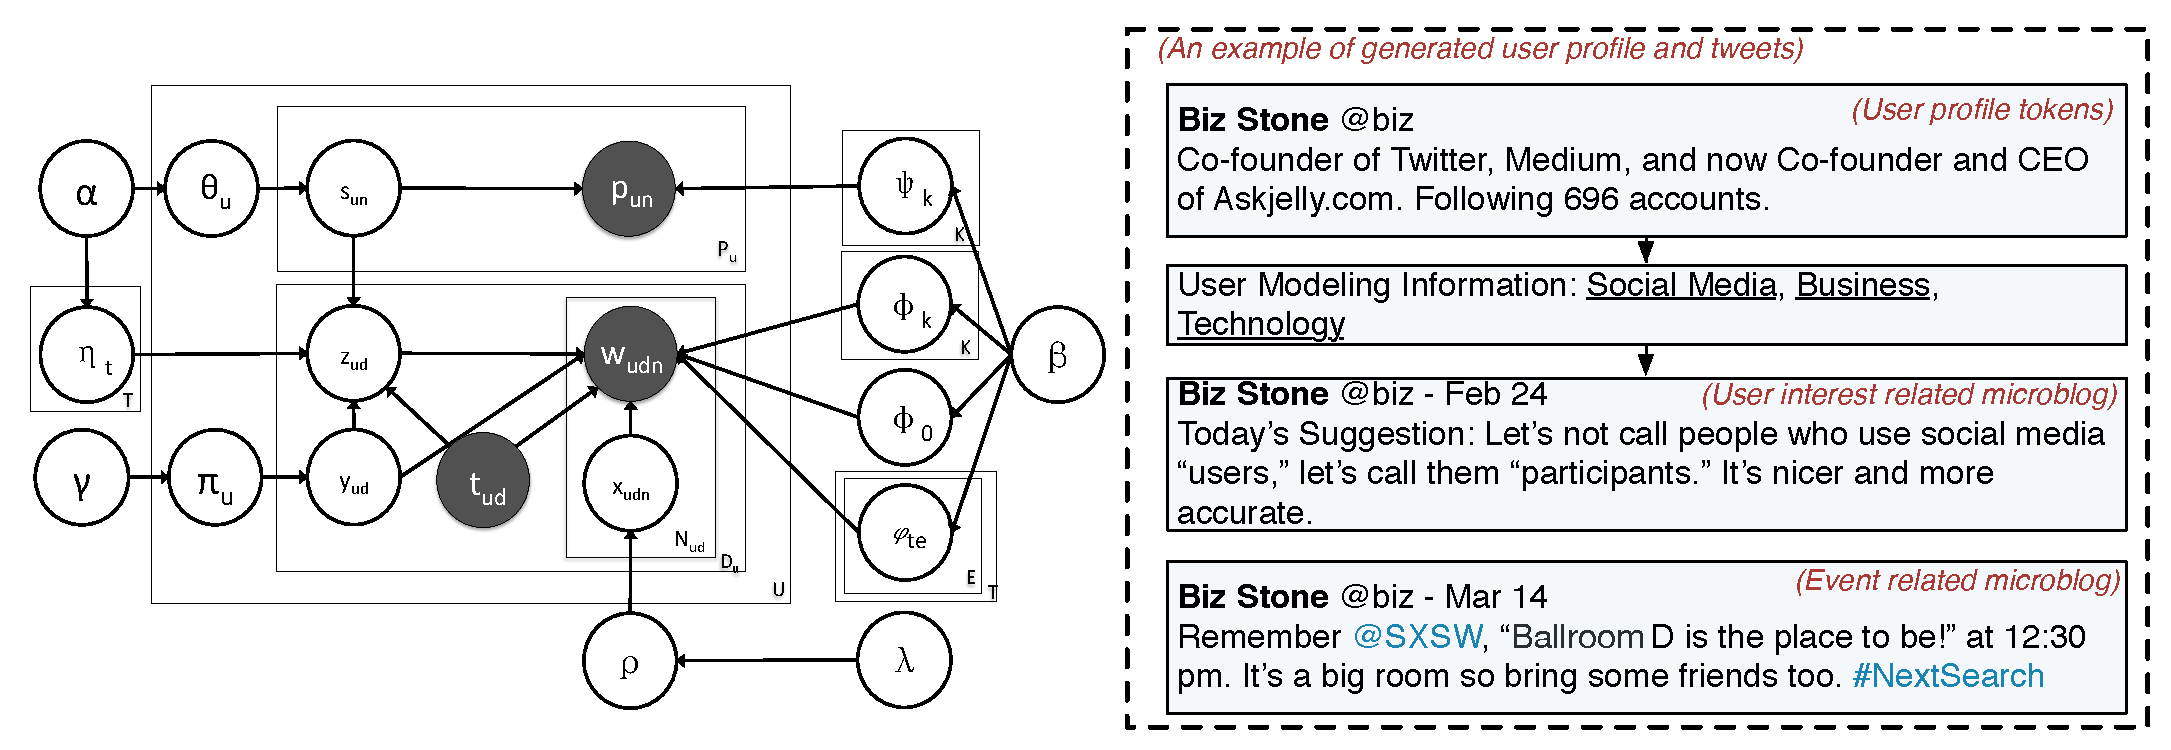
\includegraphics[width=1.0\textwidth]{img/UMIETM/model.pdf}
	\label{fig:modelUMIETM}
\end{figure}
\pdfnote{(左侧)UMIETM概率模型示意图。(右侧)示例用户Biz Stone的两类文本(用户兴趣相关的文本与突发事件相关的文本)的示意图。其个人简档揭示出其个人兴趣主要集中在社交网络、商业、科技领域。依据UMIETM模型,可以检测出他2016年2月24日发布的有关社交网络中用户角色定位的文本可以被检测为与个人兴趣相关;2016年3月14日发布的有关SXSW的文本则与个人兴趣都不相关,结合该时间窗口内更多的其他文本,可以将判断这条文本和突发事件相关,事实上SXSW是一个在3月11日到20日之间举行的盛大音乐节。}
\end{frame}

%------------------------------
\begin{frame}
\frametitle{UMIETM知识迁移算法}

\begin{columns}
\begin{column}[T]{0.42\paperwidth}
1. 根据用户个人描述信息以及关注网络计算用户兴趣分布:
\setlength{\abovedisplayskip}{1pt}
\setlength{\belowdisplayskip}{1pt}
\begin{equation}
\tiny
\label{timeUserTagLDAIVsamplingForS}
\begin{aligned}
&p(s_{un}=k|s_{\neg{un}},\vec{p},\alpha,\beta)\\
&\propto \frac{c^{(p)}_{uk}+\alpha}{c^{(p)}_{u,.}+K\alpha}
\frac{c^{(p)}_{kv}+\beta}{c^{(p)}_{k,.}+V\beta}\\
\end{aligned}
\end{equation}

2. 用户兴趣知识迁移至社交媒体文本内容中:
\begin{itemize}
	\item 和突发事件相关 
\begin{align*}
\tiny
\begin{aligned}
&p(y_{ud}=0,z_{ud}=k|\vec{y}_{\neg{ud}},\vec{z}_{\neg{ud}},\vec{t},\vec{w},\vec{s},\alpha,\beta,\gamma)\\
\end{aligned}
\end{align*}
	\item 和用户兴趣相关
\begin{align*}
\tiny
\begin{aligned}
&p(y_{ud}=1,z_{ud}=e|\vec{y}_{\neg{ud}},\vec{z}_{\neg{ud}},\vec{t},\vec{w},\vec{s},\alpha,\beta,\gamma)\\
\end{aligned}
\end{align*}

\end{itemize}

\end{column}

\begin{column}[T]{0.46\paperwidth}
\scalebox{0.65}{
\begin{minipage}{.7\paperwidth}
\begin{algorithm}[H]
\begin{spacing}{0.8}
	%\scriptsize
    \caption{UMIETM知识迁移算法} %title
    \label{alg:UMIETM_batch} %label
    \DontPrintSemicolon
    initiate the topic label and the statistics \\
    \For {\(i=1:I_1\)}{
        	\For{\(u\) in  user set \(\mathcal{U}\)}{
            		\For{\(n\) = \(1:P_u\)}{
                		sample profile's hidden topic \(s_{un}\), update \(s_{un}\), \(c^{(p)}_{u,k}\) and \(c^{(p)}_{k,v}\)
	            }%end of n
    	    }%end of u
    }%end of i
    \For{iteration \(i=1:I_2\)}{
        \For{\(t=1:T\)}{
            \For{\(u\) in  user set \(U_t\)}{
                \For{\(d\) = \(1: D_u\) }{
                    sample \(y_{ud}\) and \(z_{ud}\) \\
                    \If{\(y_{ud}=0\)}{
                        update \(z_{ud}\), \(y_{ud}\), \(c^{(0)}_u\), \(c^{(0)}_{u,k}\), \(c^{(0)}_{k,v}\)
                    }\Else{
                        update \(z_{ud}\), \(y_{ud}\), \(c^{(1)}_u\), \(c^{(1)}_{t,e}\), \(c^{(1)}_{t,e,v}\)
                    }
                    \For{\(n\) in \(1,\cdots,N_{ud}\)}{
                        sample \(x_{udn}\)\\
                        \If{\(x_{udn}=0\)}{
                            update \(x_{udn}\), \(M^{\rho}_0\), \(c^{(B)}_v\)
                        }\Else{
                            update \(x_{udn}\), \(M^{\rho}_1\), \(c^{(0)}_{k,v}\), \(c^{(1)}_{t,e,v}\)
                        }
                    }%end of n
                }%end of d
            }%end of u
        }%end of t
    }%end of i
\end{spacing}
\end{algorithm}
\end{minipage}
}
\end{column}
\end{columns}

%The following code is VERY VERY UGLLY, since we have to use the HARD CODE to set the points
%part 1 in algorithm
\begin{tikzpicture}[remember picture,overlay]
    \coordinate[xshift=63mm,yshift=-25.5mm] (A1) at (current page.north west);
    \coordinate[xshift=123mm,yshift=-25.5mm] (A2) at (current page.north west);
    \coordinate[xshift=123mm,yshift=-41mm] (A3) at (current page.north west);
    \coordinate[xshift=63mm,yshift=-41mm] (A4) at (current page.north west);
    \draw[fill=red, draw=red, opacity=0.2] (A1) -- (A2) -- (A3) -- (A4) -- (A1);
    
    \coordinate[xshift=53mm,yshift=-26mm] (s1) at (current page.north west);
	\path[->] (s1) edge [out=0, in=-180] (A1);
\end{tikzpicture}

%part 2 in algorithm
\begin{tikzpicture}[remember picture,overlay]
    \coordinate[xshift=63mm,yshift=-43mm] (B1) at (current page.north west);
    \coordinate[xshift=123mm,yshift=-43mm] (B2) at (current page.north west);
    \coordinate[xshift=123mm,yshift=-89mm] (B3) at (current page.north west);
    \coordinate[xshift=63mm,yshift=-89mm] (B4) at (current page.north west);
    \coordinate[xshift=52mm,yshift=-25mm] (s1) at (current page.north west);
    \draw[fill=blue, draw=blue, opacity=0.2] (B1) -- (B2) -- (B3) -- (B4) -- (B1);
    
    \coordinate[xshift=30mm,yshift=-50mm] (s2) at (current page.north west);
    \path[->] (s2) edge [out=0, in=270] (B1);
\end{tikzpicture}
\pdfnote{两阶段进行吉布斯采样}
\end{frame}


%------------------------------
\begin{frame}
\frametitle{UMIETM模型在线学习,提升突发事件检测时效性}
\vspace{-6mm}
\begin{columns}
\begin{column}{0.48\paperwidth}
	\begin{figure}
		\setlength{\abovecaptionskip}{0.cm}
		\setlength{\belowcaptionskip}{0.cm}
		\caption{UMIETM批量学习中遍历一轮}
		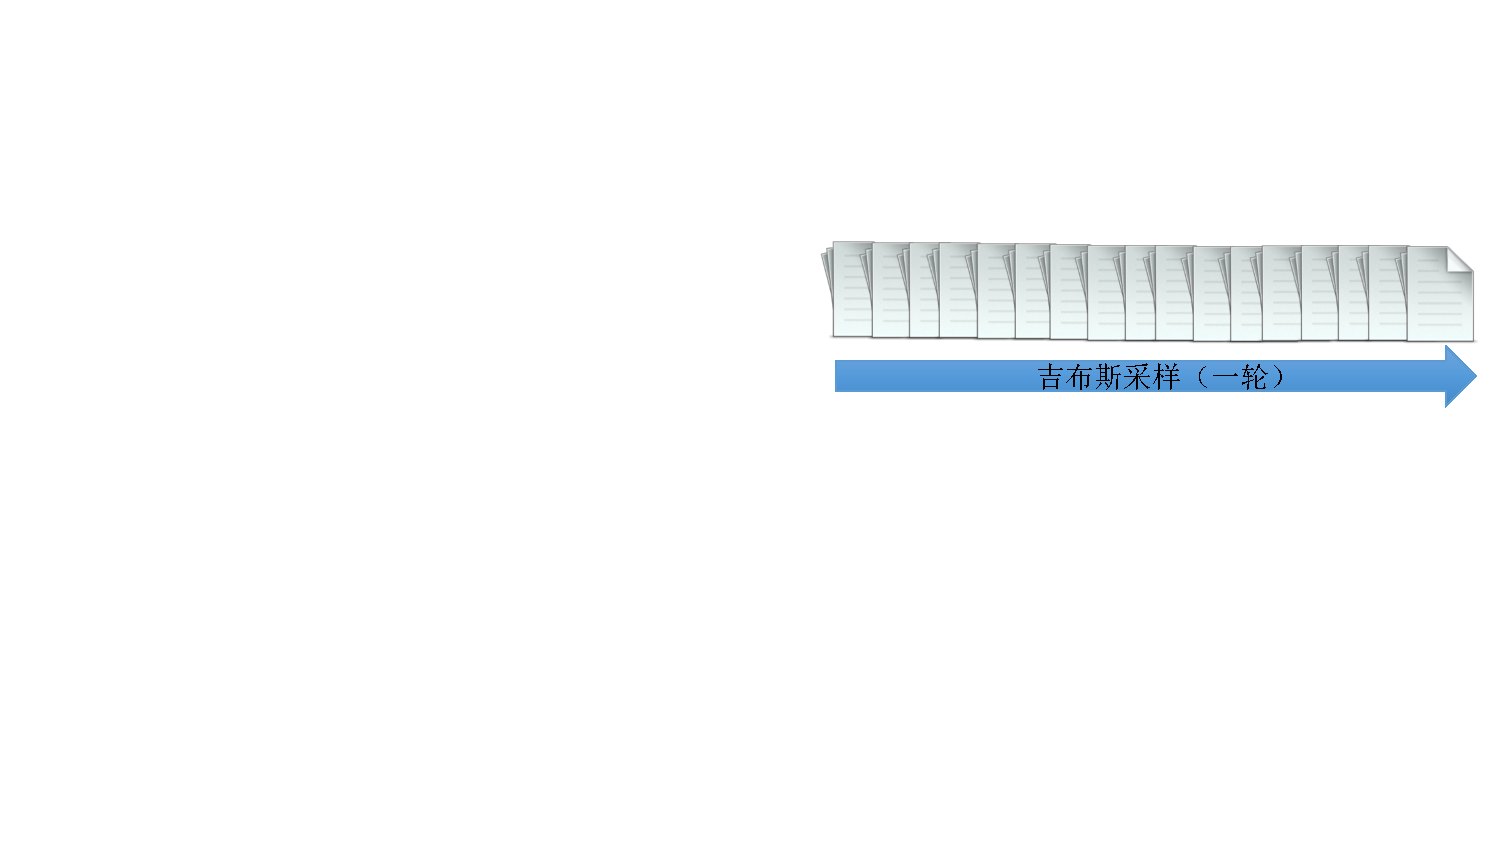
\includegraphics[width=\textwidth]{img/UMIETM/batch_learning.pdf}
	\end{figure}
\end{column}

\begin{column}{0.48\paperwidth}
	\begin{figure}
		\setlength{\abovecaptionskip}{0.cm}
		\setlength{\belowcaptionskip}{0.cm}
		\caption{UMIETM在线学习提升效率}
		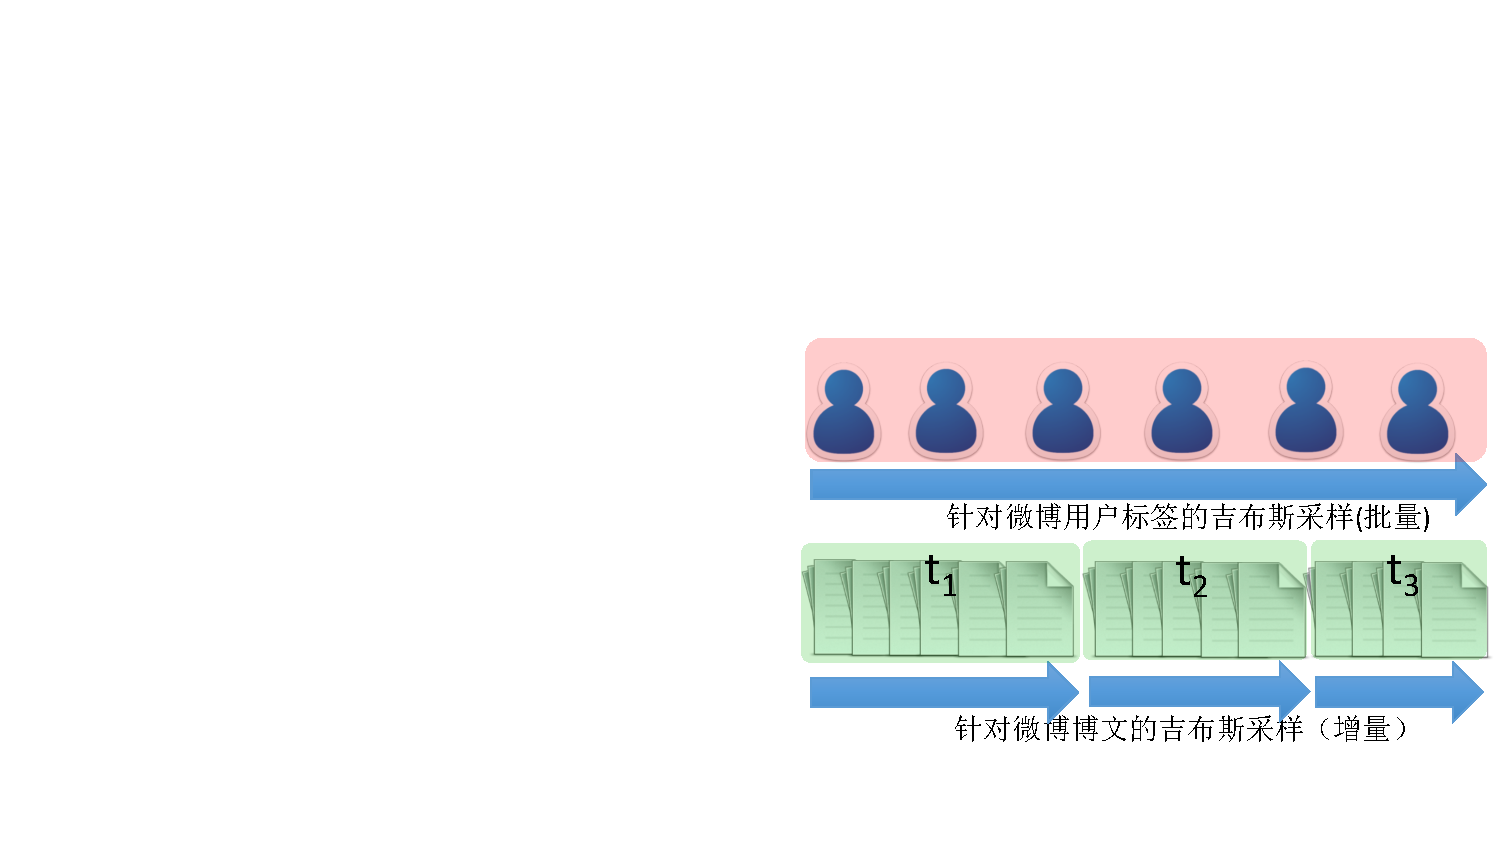
\includegraphics[width=\textwidth]{img/UMIETM/online_learning.pdf}
	\end{figure}
\end{column}	
\end{columns}

\vspace{-1mm}

\begin{table}[ht]
	\setlength{\abovecaptionskip}{0.cm}
	\setlength{\belowcaptionskip}{0.cm}
	\caption{UMIETM批量学习与在线学习时间复杂度与空间复杂度对比表,其中\(|W_t| \ll |W|\)}
	\begin{tabular}{|l|c|c|}
	\hline
       & 时间复杂度 & 空间复杂度 \\ \hline
	UMIETM批量学习方法  & \(O(I_1 K|P|+I_2 (K+E)|W|)\) & \(O(|P|+|W|)\) \\ \hline
	UMIETM在线学习方法 & \(O(I_1 K|P|+I_2 (K+E)|W_t|)\) & \(O(|P|+|W_t|)\) \\
	\hline
	\end{tabular}
\end{table}


\end{frame}

%------------------------------
\begin{frame}
\frametitle{UMIETM对社交媒体动态语境演变的自适应}
社交媒体的语境动态演变不断带来新词,新词也意味着新的事件,UMIETM需要相应自适应机制。

\begin{figure}
	\centering
	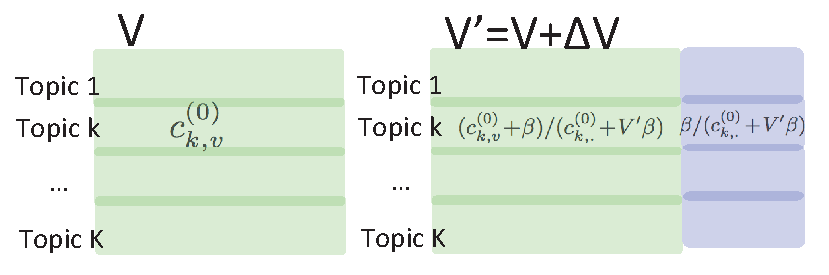
\includegraphics[height=3.1cm]{img/UMIETM/stream2.pdf}
	\caption{社交媒体数据流上新增的词汇采用smoothing的方式初始化}
\end{figure}
\end{frame}

%------------------------------
\begin{frame}
\frametitle{实验设置(1/2)}
\begin{itemize}
	\item 新浪微博数据集2012.1.1-2012.12.31
	\item 数据预处理
	\begin{enumerate}
		\item 数据集按周进行分割,得到时间窗口文件
		\item 中文分词(ICTCLAS 2013)
		\item 移除停用词与低频词(时间窗口内文档频度<3)
		\item 移除过短的微博文本(词数<3)
	\end{enumerate}
\end{itemize}

\begin{table}
\setlength{\abovecaptionskip}{0.cm}
\setlength{\belowcaptionskip}{0.cm}
\scriptsize
\centering
\caption{预处理后的新浪微博数据集上的统计信息}
\begin{tabular}{|c|r|r|r|} \hline
 & 用户数 & 微博数 & 微博中词的数量 \\ \hline
全年& 252,369 & 16,421,167 & 251,686,571\\ \hline
第1周 & 9,785 & 31,503 & 440,217 \\ \hline
第2周 & 29,721 & 242,554 & 3,679,979 \\ \hline
第3周 & 30,891 & 254,698 & 3,881,633 \\ \hline
第4周 & 29,788 & 237,456 & 3,510,934 \\ \hline
第5周 & 24,256 & 190,037 & 2,749,539 \\ \hline
\(\dots\) & \(\dots\) & \(\dots\) & \(\dots\) \\ \hline
\end{tabular}
\label{statisticsOfDataset}
\end{table}
\pdfnote{这一页的实验说明检验模型有效性}
\end{frame}

%------------------------------
\begin{frame}
\frametitle{实验设置(2/2)}

\begin{itemize}
	\item 社交媒体数据流Large twitter corpus(相比于Edinburgh twitter corpus):
	\begin{itemize}
		\item 61,2091,163条微博
		\item 7,695,256个用户
		\item 时间跨度:2011年7月1日到2011年12月18日。
		\item 以10分钟为单位进行数据分片。
	\end{itemize}
	\item 突发事件基准:Wikipedia上用户整理的事件列表2011 in the United States\#Events\footnote{\url{https://en.wikipedia.org/wiki/2011_in_the_United_States\#Events}},43个突发事件。
\end{itemize} 
\pdfnote{这一页的实验说明检验模型的时效性\\ 是否要说是在MALLET上实现UMIETM算法,并在8核的2.00HZ,64GB内存的服务器上运行。}
\end{frame}

%------------------------------
\begin{frame}
\frametitle{实验结果:UMIETM模型有效性}	
\begin{itemize}
	\item 对比方法:Author-LDA, twitterLDA, timeUserLDA,以及不使用用户个人描述信息进行用户建模的变体方法IETM
	\item 度量指标:困惑度(perplexity)
\end{itemize}
\begin{equation}
\label{eq:UMIETM_perplexity}
perplexity(D_{test})=\exp{\{-\frac{\sum_{u=1}^{U}\sum_{d=1}^{D_u}\log{p(w_{ud})}}{\sum_{u=1}^{U}\sum_{d=1}^{D_u}N_{ud}}\}}
\end{equation}

%\begin{equation}
%\scriptsize
%\begin{aligned}
%\label{eq:UMIETM_p_w_ud}
%&p(w_{ud})=(1-\pi_u)\sum_{k=1}^{K}\theta_{uk}\prod_{n=1}^{N_{ud}}(\phi_{s,w_{udn}}(1-\rho)+\phi_{k,w_{udn}}\rho)+\\
%&\ \ \ \ \pi_u \sum_{k=1}^{K}\eta_{t,k}\prod_{n=1}^{N_{ud}}(\phi_{s,w_{udn}}(1-\rho)+\phi_{k,w_{udn}}\rho)
%\end{aligned}
%\end{equation}

\begin{table}
\centering
\caption{UMIETM与对比方法的困惑度比较(数值较小者文本建模的有效性更强)}
\begin{tabular}{|c|r|r|r|r|} \hline
Author-LDA & TwitterLDA & TimeUserLDA & IETM & UMIETM\\ \hline
20422.25 & 6027.47 &  4810.92 & 3926.76 & 3107.83\\ \hline
\end{tabular}
\label{tab:heldoutPerplexity}
\end{table}
\pdfnote{1,从表中可以看出IETM和UMIETM都比其他方法更优,说明区分用户兴趣与突发事件有助于提升文本建模效果;\\ 2,而UMIETM比IETM更优,说明通过用户个人简档和关注网络信息进行的建模比单纯建模社交媒体文本更优。}
\end{frame}

%------------------------------
\begin{frame}
\frametitle{实验结果:UMIETM算法收敛速度}
\begin{figure}
	\caption{UMIETM迭代10次之后,完全对数似然函数值的增长幅度小于0.15\%}
    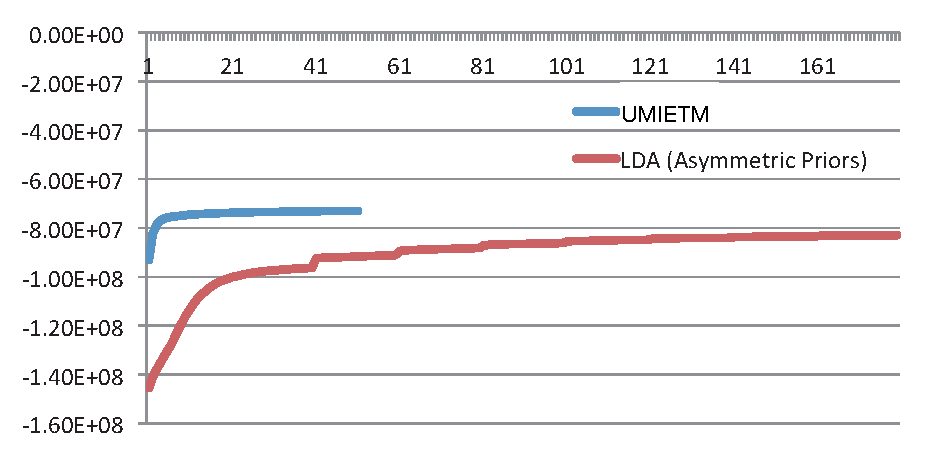
\includegraphics[width=1.0\textwidth]{img/UMIETM/completeLoglikelihood.pdf}
\end{figure}

\end{frame}


%------------------------------
\begin{frame}
\frametitle{实验结果:UMIETM事件检测效率}
\begin{figure}
	\caption{UMIETM在线学习方法用于事件检测的运行效率}
    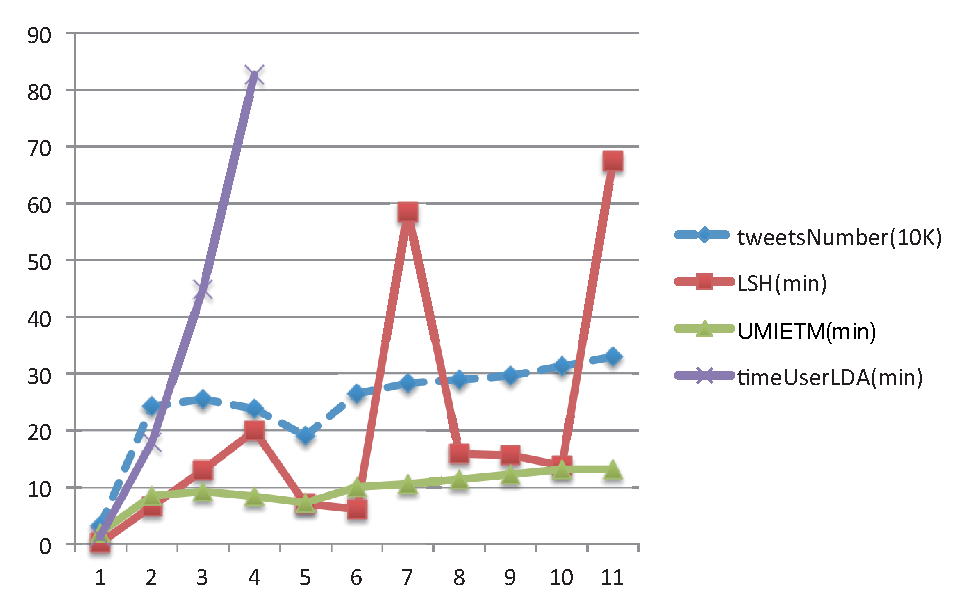
\includegraphics[width=0.8\textwidth]{img/UMIETM/efficiencyCompareWithLSH.pdf}
\end{figure}
\pdfnote{timeUserLDA使用批量学习方法,时间复杂度随着数据集大小线性增长\\ 基于LSH的方法也具备在线学习能力,但时间复杂度不稳定,随着桶内数据大小而变化}
\end{frame}

%------------------------------
\begin{frame}
\frametitle{实验结果:突发事件检测准确率与召回率}

\begin{table}
\centering
\caption{UMIETM与对比方法在新浪微博数据集(2012.1-2012.12)上突发事件检测任务的准确率与召回率比较}
\begin{tabular}{|c|c|c|c|} \hline
 & precision & recall & F \\ \hline
UMIETM & 0.894 & 0.913 & 0.903\\ \hline
UMIETM(-) & 0.847 & 0.697 & 0.765\\ \hline
IETM & 0.824 & 0.536 & 0.650\\ \hline
LSH & 0.394 & 0.913 & 0.550\\ \hline
EDCoW & 0.731 & 0.435 & 0.545\\ \hline
\end{tabular}
\label{tab:metrics}
\end{table}
\pdfnote{注意是否要增加一个Twevent的实验,或者我们要不要增加一个新的结果(最好是2016或者2017的)}
\end{frame}

%------------------------------
\begin{frame}
\frametitle{实验结果:社交媒体数据流中检测突发事件时效性}
\vspace{-6mm}
\begin{table}
\setlength{\abovecaptionskip}{0.cm}
\setlength{\belowcaptionskip}{0.cm}
\centering
\caption{\textit{Large twitter corpus}数据集中的突发事件}
\label{my-label}
\scalebox{0.50}{
\begin{threeparttable}  
\begin{tabular}{|c|l|c|c|c|}
\hline
\multirow{2}{*}{Date}  & \multirow{2}{*}{Representative event tweet} & \multicolumn{3}{c|}{Methods\tnote{a}} \\ \cline{3-5} 
 &  & LSH  & TW & UMIETM \\ \hline
9/17/11  & \begin{tabular}[c]{@{}l@{}l@{}} Day of \textbf{Rage} \textbf{occupies Wall Street} Democracy in Action!\\ Watching globalrevolution http://livestre.am/PlNN  via\\ @livestream \end{tabular} & 4:10PM & 3:50PM & 3:30PM \\ \hline
 ... & ... & ... & ... & ... \\ \hline
11/4/11  & \begin{tabular}[c]{@{}l@{}l@{}}Hotmail - mikehuot@msn.com - Windows Live\\ http://bit.ly/vRDssg  via @addthis \textbf{Andy Rooney}'s\\ Essay on Prayer! Gonna \textbf{miss} that old man! \end{tabular} & 11:20PM & 9:10PM & 7:30PM \\ \hline
11/7/11 & \begin{tabular}[c]{@{}l@{}}\textbf{Jerry Sandusky} Accused Of \textbf{Sexually Assaulting} 8 \textbf{Boys}.. \end{tabular} & 4:50PM & 4:20PM & 4:00PM  \\ \hline
11/8/11  & \begin{tabular}[c]{@{}l@{}l@{}} Here, I'm going to declare \textbf{Phil Bryant} a winner in the \\ Mississippi gubernatorial \textbf{race} right now. Take that, CNN. \end{tabular} & - & - & 1:40PM \\ \hline
11/8/11 & \begin{tabular}[c]{@{}l@{}l@{}l@{}l@{}} Miss. \textbf{voters} asked if life begins at \textbf{conception}: JACKSON,\\ Miss. (AP) -- \textbf{Mississippi voters} were asked Tuesda... \\http://apne.ws/sjgCMh \end{tabular} & 10:00PM &  12:20PM & 11:50AM \\ \hline
11/8/11 & \begin{tabular}[c]{@{}l@{}l@{}l@{}l@{}} Looks like \textbf{Steve Beshear} is going to easily win \textbf{reelection}! \end{tabular} & - & 4:50PM  & 3:50PM \\ \hline
11/8/11 & \begin{tabular}[c]{@{}l@{}l@{}l@{}l@{}} Will \textbf{Republicans} seize control of the \textbf{Virginia state Senate}?\\ So far, our readers say yes. http://patch.com/A-n6G7  \\ What do you think? \#va31 \end{tabular} & - & 4:40PM  & 3:20PM \\ \hline
11/8/11 & \begin{tabular}[c]{@{}l@{}l@{}l@{}l@{}} Is it the end of \textbf{Russell Pearce}'s future as state senator? \\ \textbf{Recall Vote} today. - http://bit.ly/tZHNMn \end{tabular} & - & 2:40PM  & 1:30PM \\ \hline
... & ... & ... & ... & ... \\ \hline
12/18/11 & \begin{tabular}[c]{@{}l@{}l@{}l@{}l@{}} The \textbf{iraq war} is \textbf{over}, but the war on Iran is just beginning \end{tabular} & 11:20AM & 9:50AM  & 9:30AM \\ \hline
\end{tabular}

\begin{tablenotes}  
\item[a] LSH, TW=Twevent
\end{tablenotes}  
\end{threeparttable}  
}
\label{tbl:bursty_events_timeliness}
\end{table}
\footnote{以事件\textit{占领华尔街运动}为例,由新闻报道可知在2011年9月17日下午3点“占领华尔街运动”的抗议人群开始聚集在华尔街铜牛处。表显示UMIETM模型能够半个小时之后就检测到此突发事件。\\ 另一个例子是,2011年12月18日,美国从伊拉克撤出最后一批驻军,UMIETM能够在早上9点30分就检测到这一突发事件,而LSH方法则迟至中午11点20才检测到突发事件。}
\end{frame}

%------------------------------
%\begin{frame}
%\frametitle{实验结果:社交媒体数据流中检测突发事件时效性}	
%
%\pdfnote{43个突发事件平均提前1.4小时检测}
%\end{frame}

%------------------------------
\begin{frame}
\frametitle{UMIETM方法小结}	
\begin{columns}
\column{0.75\textwidth}

\begin{enumerate}
	\item 提出了一种用户兴趣建模与知识迁移方法UMIETM,检测社交媒体突发事件;
	\item 使用用户个人描述信息与关注网络,建模用户兴趣并迁移到社交媒体文本中,区分用户个人兴趣相关的文本和由外部突发事件引起的文本;
	\item 将UMIETM扩展为在线学习的方式,应用于实际的社交媒体数据流;
	\item 相较于已有方法能够提前1.4小时检测突发事件
\end{enumerate}

\column{0.25\textwidth}

\end{columns}

\pdfnote{1,本文提出了一种用户兴趣建模与知识迁移方法UMIETM,检测社交媒体突发事件。\\ 2,UMIETM使用用户个人描述信息与关注网络,学习出用户个人兴趣,并将用户个人兴趣的知识迁移到社交媒体数据流中,区分用户个人兴趣相关的文本和由外部突发事件引起的文本。\\ 3,将UMIETM扩展为在线学习的方式,应用于实际的社交媒体数据流。\\ 4,相较于已有方法能够提前1.4小时检测突发事件}
\end{frame}
